\documentclass[10pt]{beamer}
\usepackage{colortbl,verbatim}
\usepackage{multirow}
\usepackage{colortbl}
\usepackage{rotating}
\usepackage[absolute,overlay]{textpos}
\newenvironment{enumwide}%
{\begin{enumerate}%
    \setlength{\itemsep}{5pt}%
    \setlength{\parskip}{5pt}}%
  {\end{enumerate}}
\newenvironment{itemwide}%
{\begin{itemize}%
    \setlength{\itemsep}{5pt}%
    \setlength{\parskip}{5pt}}%
  {\end{itemize}}


\mode<presentation>
{
  %\usetheme{Warsaw}
  %\usetheme{Montpellier}
  \usetheme{Singapore}
  %\usecolortheme{crane}
  %\usecolortheme{seahorse}
  \setbeamercovered{transparent}
}

%   \usetheme{default}
%   \usecolortheme{seahorse}
%   \setbeamerfont{alerted text}{series=\bfseries}

%%\pgfdeclareimage[height=0.85cm]{bmlogo}{/home/bart/presentation_relextraction/pics/Logo_BM_EN.pdf}
\pgfdeclareimage[height=0.85cm]{bmlogo}{pics/Logo_BM_EN}

\title{Opinion Mining of Spanish Customer Comments with Non-Expert Annotations on\\ Mechanical Turk}

\author{Bart Mellebeek, Francesc Benavent, Jens Grivolla,\\ Joan Codina, Marta Ruiz and Rafael Banchs}

\institute
{
  Barcelona Media Centre d'Innovacio\\ \vspace{.2cm}
  \pgfuseimage{bmlogo}
}

\date{Barcelona, \today}

\AtBeginSection[]
{
   \begin{frame}
       \frametitle{Outline}
       \tableofcontents[currentsection]
   \end{frame}
}
\begin{document}

\frame{\titlepage}

\begin{frame}
  \frametitle{Outline}
  \tableofcontents
\end{frame}

\section{What is Mechanical Turk?}

\begin{frame}
  \frametitle{Who was \textit{The Turk}?}
  \begin{center}
    \scalebox{.4}{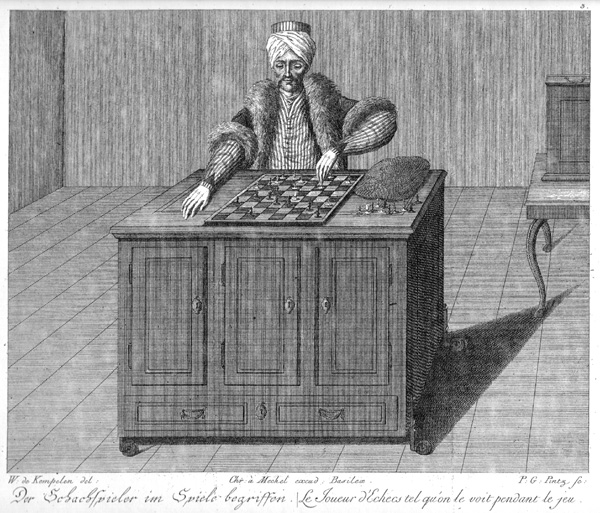
\includegraphics{pics/Turk-engraving5.jpg}}
  \end{center}
\end{frame}

\begin{frame}
  \frametitle{Who was \textit{The Turk}?}
  \begin{center}
    \scalebox{.4}{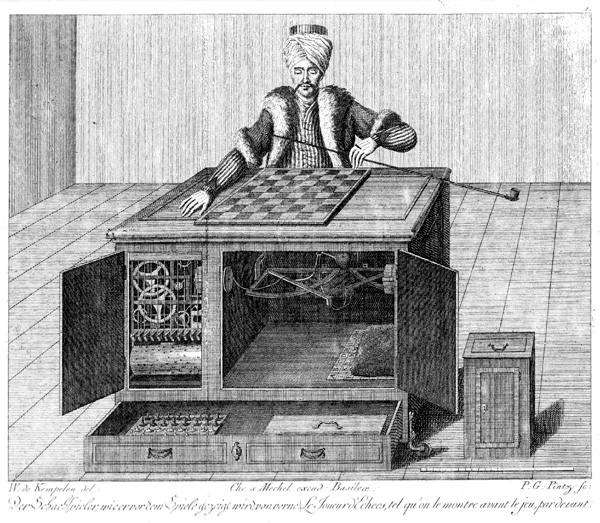
\includegraphics{pics/Turk-engraving6.jpg}}
  \end{center}
\end{frame}

\begin{frame}
  \frametitle{Who was \textit{The Turk}?}
  \begin{center}
    \scalebox{.4}{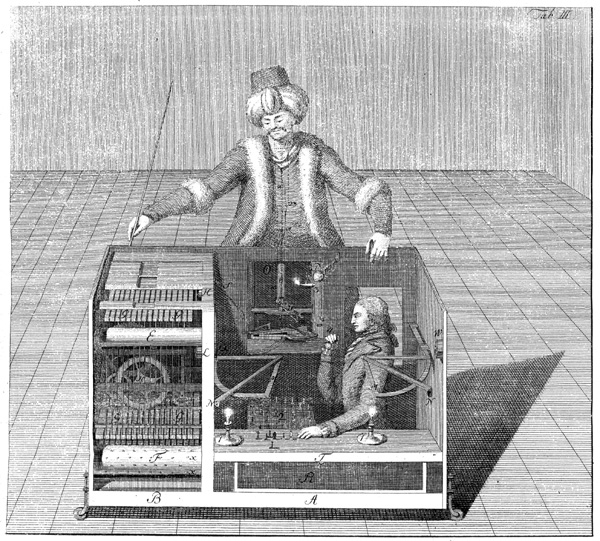
\includegraphics{pics/Turk-engraving7.jpg}}
  \end{center}
\end{frame}

\begin{frame}
  \frametitle{Amazon Mechanical Turk (AMT) $=$ \textit{artificial} Artificial Intelligence}
	\begin{itemwide}
 	\item Human annotations are a bottleneck for data-driven AI Systems.
	\item Amazon Mechanical Turk (AMT) is a marketplace for work.
	\item HIT $=$ Human Intelligence Task.
	\item AMT workers can choose between tens of thousands of different HITs at whichever time they want.
	\item AMT requesters have access to a global workforce.
	\item Crowdsourcing $\rightarrow$ other platforms such as \textit{Crowdflower}
	\end{itemwide}
\end{frame}

\begin{frame}
  \frametitle{Is Mechanical Turk a sweatshop?}
  \begin{center}
    \scalebox{.45}{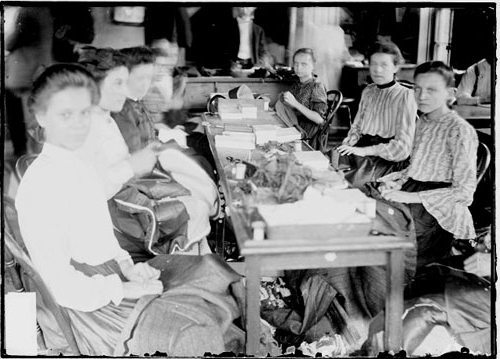
\includegraphics{pics/1903sweatshopchicago.jpg}}
  \end{center}
\end{frame}

\begin{frame}
  \frametitle{Is Mechanical Turk a sweatshop?}
\begin{columns}[T]
\begin{column}{5cm}
\scalebox{.5}{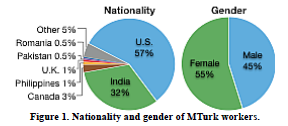
\includegraphics{pics/geography.png}}

\begin{footnotesize}
\begin{tabular}{p{4cm}}
\\ \\ \\ \\ \\ \\ \\ \\ \\ \\ \\
 Ref: Who are the Turkers? Worker Demographics in Amazon Mechanical Turk. Ross et al, 2009.
\end{tabular} 
\end{footnotesize}
\end{column}
\begin{column}{5cm}
\scalebox{.5}{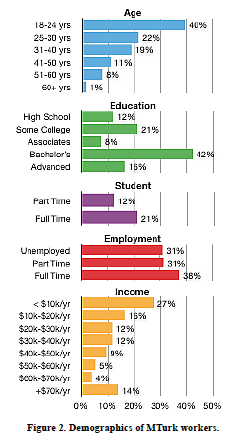
\includegraphics{pics/demographics.png}}
\end{column}
\end{columns}
\end{frame}

\begin{frame}
  \frametitle{AMT worker annotations are cheap and fast. Are they also good?}
	\begin{itemwide}
 	\item A number of recent papers argue they are: Kittur et al. (2008), Snow et al. (2008), Mason and Watts (2009), $\ldots$
	\item Highly dependent on type of task.
	\item General conclusion: the combination of several AMT worker annotations is better and cheaper than the annotations of a single expert.
	\end{itemwide}
\end{frame}

\section{Task Outline and Goals}

\begin{frame}
  \frametitle{Task Outline}
\begin{itemwide}
 \item NAACL 2010 Workshop: Creating Speech and Language Data With Amazon's Mechanical Turk.
 \item Shared Task: What can you do with \$100 and Amazon Mechanical Turk?
 \item Participants share data \& HIT templates.
\end{itemwide}

\end{frame}

\begin{frame}
  \frametitle{Goals}
We compare different HIT design strategies by evaluating the usefulness of resulting Mechanical Turk (AMT) annotations to train an Opinion Mining System on Spanish consumer data.\\

\vspace{1cm}

\begin{block}{Research questions:}
 \begin{enumerate}
 \item Annotation quality: AMT workers vs. experts.
 \item Annotation applicability: training of batch of classifiers.
 \item Language barriers: is there a large enough worker pool for Spanish?
 \item Return on Investment: AMT workers vs. experts.
\end{enumerate}
\end{block}

\end{frame}

\section{HIT Design}

\begin{frame}
  \frametitle{HIT $=$ Human Intelligence Task}
  \begin{center}
    \scalebox{.2}{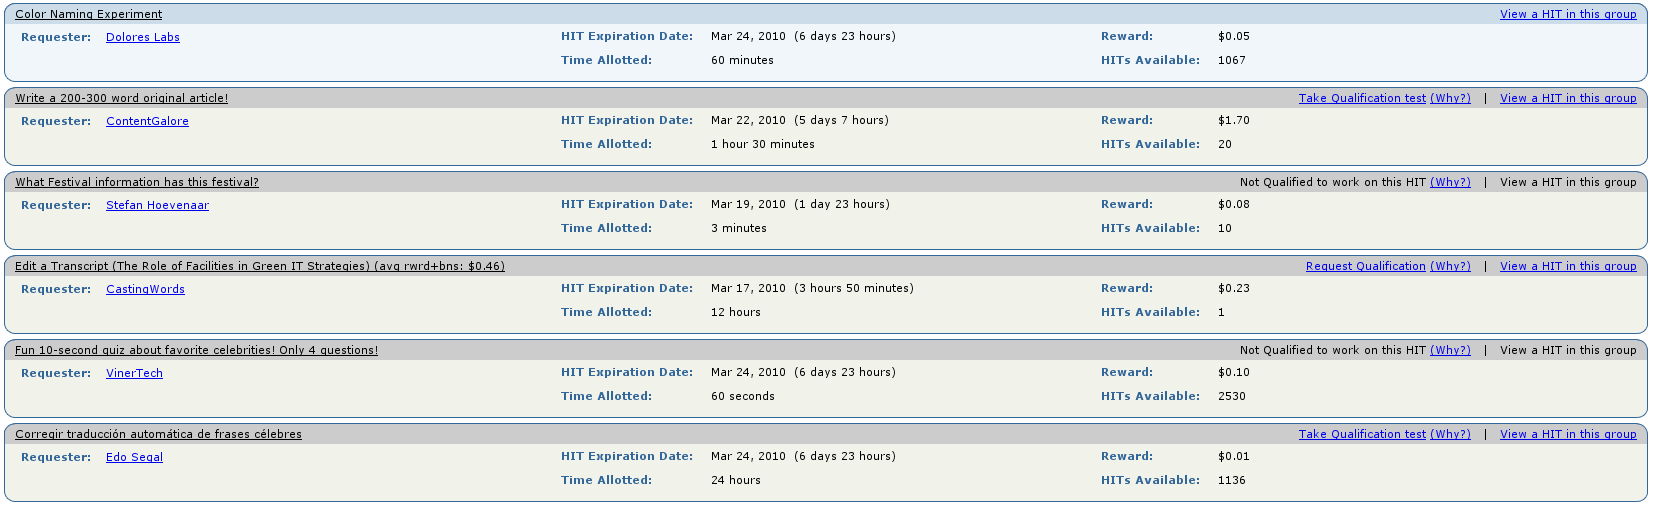
\includegraphics{pics/HIT_example.png}}
  \end{center}
\end{frame}

\begin{frame}
  \frametitle{Source of our data: \texttt{www.ciao.es}}

All sentences were extracted from a corpus of user opinions on cars from the automotive section of \texttt{www.ciao.es}.

  \begin{center}
    \fbox{
    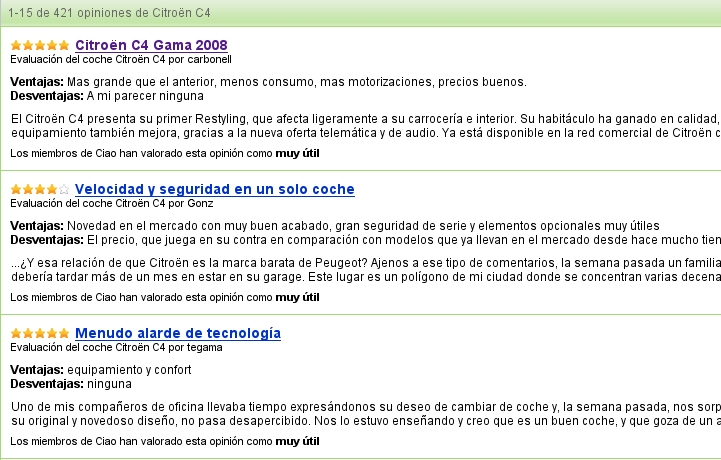
\includegraphics[scale=0.4]
	{pics/ciao.png}}
  \end{center}

\end{frame}

\begin{frame}
  \frametitle{\texttt{www.ciao.es}: some example sentences}
\begin{itemwide}
 \item ¡No te lo pienses m\'{a}s, c\'ompratelo!
 \item Tiene muchas piezas defectuosas.
 \item La conducci\'{o}n es genial pero el diseño una porquer\'{i}a.
 \item El Volvo es mejor que el Fiat.
 \item Este coche tiene 6 cilindros.
\end{itemwide}


\end{frame}

\begin{frame}
  \frametitle{HIT Design}
  \begin{center}
    \fbox{
    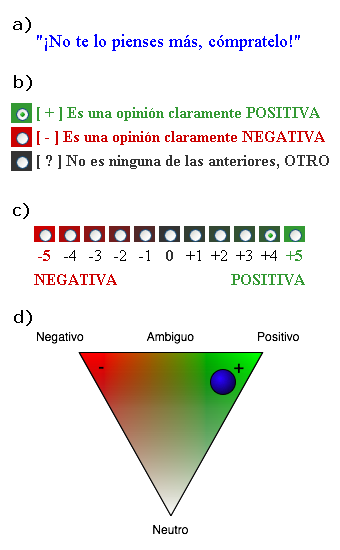
\includegraphics[scale=0.4]
	{pics/Reshots_All.png}}
  \end{center}
\end{frame}

\begin{frame}
  \frametitle{Competence Test}
\begin{itemwide}
 \item Uploaded test batch of 30 HITs.
 \item Performed in matter of minutes but $\ldots$
 \item most answers were random clicks.
\end{itemwide}
\end{frame}

\section{Annotation Results}

\begin{frame}
  \frametitle{HIT Statistics}
\begin{center}
\begin{small}
\begin{tabular}{|l|l|c|c|c|c|c|c|c|}
 \hline
 \multicolumn{3}{|c|}{Overall} & \multicolumn{2}{|c|}{HIT1} & \multicolumn{2}{|c|}{HIT2} & \multicolumn{2}{|c|}{HIT3}  \\ \hline
 ID & C & \% & \# & sec. & \# & sec. & \# & sec. \\ \hline %A1VZZ0Z066Y4Z6
 1 & mx & 29.9 & 794 & 11.0 & 967 & 8.6 & 930 & 11.6 \\ %A198YDDSSOBP8A
 2 & us & 27.6 & 980 & 8.3 & 507 & 7.8 & 994 & 7.4 \\ %A1F70TQGR00PTQ
 3 & nl & 11.0 & 85 & 8.3 & 573 & 10.9 & 333 & 11.4 \\ %A3GPY0YRKEQFTN
 4 & us & 9.5 & 853 & 16.8 & - & - & - & - \\ %A1VZZ0Z066Y4Z6
 5 & es & 9.4 & - & - & 579 & 9.1 & 265 & 8.0 \\ %A36Y503MT333BI
 6 & ec & 4.1 & 151 & 9.4 & 14 & 16.7 & 200 & 13.0 \\ %A28EP28N6ZVN92
 7 & us & 3.6 & 3 & 15.7 & 139 & 8.5 & 133 & 11.6 \\ %A1COK1GRYUJA1M
 8 & us & 2.2 & 77 & 8.2 & 106 & 7.3 & 11 & 10.5 \\ %A16MC82ITK70QZ
 9 & us & 0.6 & - & - & - & - & 50 & 11.2 \\ %AMFD4SECCGB9M
 10 & us & 0.5 & 43 & 5.3 & 1 & 5 & - & - \\ %A19835WFUL4B52
 11 & us & 0.4 & - & - & 38 & 25.2 & - & - \\ %AKZL93LN5PNM8
 12 & us & 0.4 & - & - & 10 & 9.5 & 27 & 10.8 \\ %A1CY631WJA8W0F
 13 & es & 0.4 & - & - & - & - & 35 & 15.1 \\ %A2RUNAAB6696MJ
 14 & es & 0.3 & - & - & 30 & 13.5 & - & - \\ %A14OKIBGWHJE1F
 15 & us & 0.3 & 8 & 24.7 & 18 & 21.5 & - & - \\ %A1H95IZT6SJKC9
 16 & us & 0.2 & - & - & - & - & 22 & 8.9 \\ %A3TXA8FQAXNMDM
 17 & us & 0.2 & - & - & 17 & 16.5 & - & - \\ %A2M7EYDXHMTLL7
 18 & ? & 0.1 & 6 & 20  & - & - & - & -  \\ %A6FD8TNCPBP69
 19 & us & 0.1 & - & - & 1 & 33 & - & -  \\ %A1B326VW79CZEP
 \hline
\end{tabular}
\end{small}
\end{center}
\end{frame}

\begin{frame}
  \frametitle{Annotation Distributions}
  \begin{center}
    \fbox{
    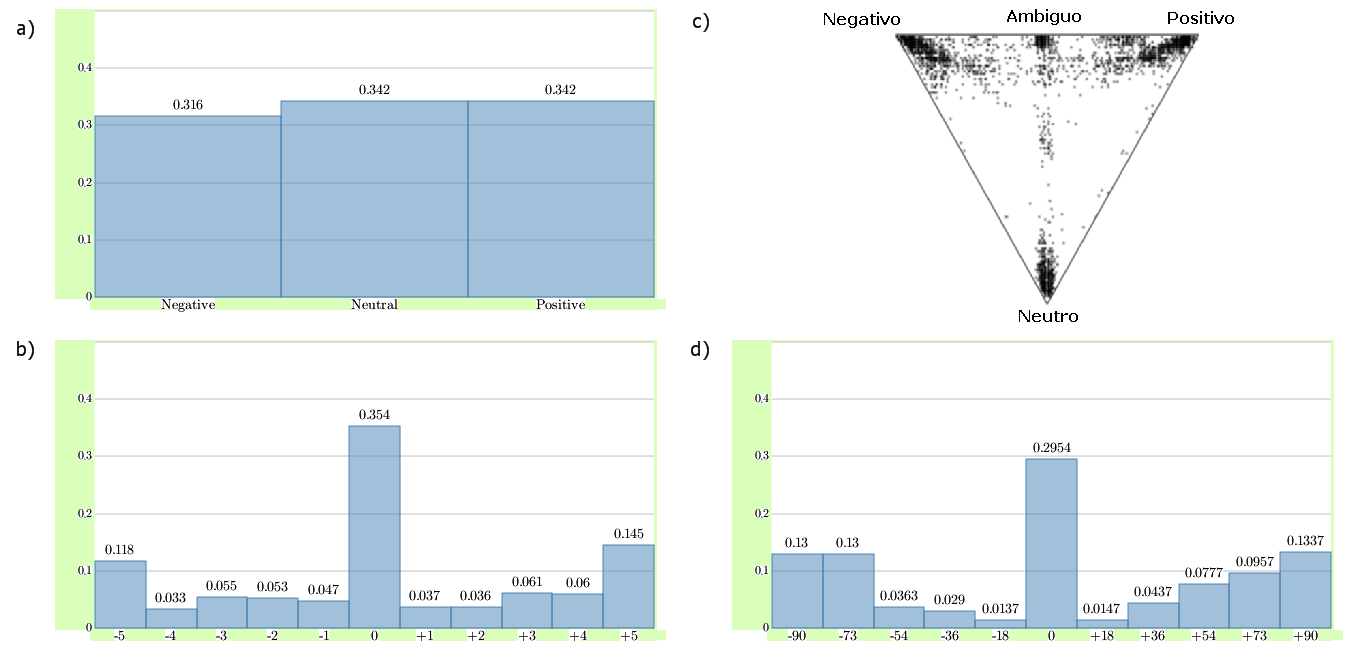
\includegraphics[scale=0.23]
	{pics/Histograms.png}}
  \end{center}
\end{frame}

\begin{frame}
  \frametitle{Annotation Quality}
\begin{center}
\begin{tabular}{|l|c|c|}
\hline
& $\kappa_{1}$ & $\kappa_{2}$ \\ 
\hline
Inter-batch & 0.598 & 0.598 \\ \hline
Batch\_1 vs. Expert & 0.628 & 0.628\\
Batch\_2 vs. Expert & 0.649 & 0.649\\
Batch\_3 vs. Expert & 0.626 & 0.626\\ \hline
Majority vs. Expert & 0.716 & 0.716\\ \hline
Experts\footnote{Results on a different 500-sentence random sample of the same corpus.} & 0.725 & 0.729\\ \hline
\end{tabular}
\end{center}
\end{frame}

\begin{frame}
  \frametitle{Annotation Costs}
\begin{itemwide}
 \item A total amount of 9000 assignments were uploaded on AMT.
 \item Reward of .02\$ per assignment $\rightarrow$ total sum $=$ 225\$ (180\$ + 45\$ Amazon fees).
 \item In-house expert: 1000 assignments in three hours at 70\$ per hour.
 \item We saved 210\$ ($= 70 \times 3$) - 75\$ ($ = \frac{225}{3}$) = 135\$, which constitutes almost 65\% of the cost of an expert annotator.
 \item + a lower reward (.01\$) would most probably have worked equally well.
\end{itemwide}

\end{frame}

\section{Experimental Results}

\begin{frame}
  \frametitle{Two Experiments}
\begin{itemwide}
 \item Experiment 1: practical utility. Train a single polarity classifier on different data sets. Compare system with noisy available metadata and with AMT generated annotations of HIT1.
 \item Experiment 2: theoretical utility. Train several polarity classifiers using the same data set, annotated by experts and AMT workers.
\end{itemwide}

\end{frame}

\begin{frame}
  \frametitle{Description of Data Sets}

All sentences were extracted from a corpus of user opinions on cars from the automotive section of \texttt{www.ciao.es}.

% \begin{itemize}
%  \item Ciao opinions are marked with a rating 1 (negative) to 5 (positive).
%  \item Baseline: 5570 sentences, roughly distributed $1/3$ positive, $1/3$ neutral and $1/3$ negative.
%  \item Annotated: 1000 sentences, roughly distributed $1/3$ positive, $1/3$ neutral and $1/3$ negative.
%  \item Evaluation: 500 sentences, roughly distributed $1/3$ positive, $1/3$ neutral and $1/3$ negative.
% \end{itemize}

\vspace{1cm}

\begin{center}
\begin{tabular}{|l|l|l|l|}
\hline
&Baseline &Annotated &Evaluation \\
\hline
Positive &1882 &341 &200 \\
\hline
Negative &1876 &323 &137 \\
\hline
Neutral &1812 &336 &161 \\
\hline
Totals &5570 &1000 &500 \\
\hline
\end{tabular}
\end{center}

\end{frame}

\begin{frame}
  \frametitle{Experiment 1}

\begin{center}
\begin{tabular}{|l|l|l|}
\hline
classifier &baseline &annotated \\ 
\hline
positive/not\_positive &59.63 (3.04) &69.53 (1.70) \\ 
\hline
negative/not\_negative &60.09 (2.90) &63.73 (1.60) \\ 
\hline
neutral/not\_neutral &51.27 (2.49) &62.57 (2.08) \\ 
\hline
\end{tabular}
\end{center}

\end{frame}

\begin{frame}
  \frametitle{Experiment 2}
\begin{center}
\begin{small}
\begin{tabular}{|l|l|l|l|l|l|l|} \hline
 System & 
 {\begin{sideways}\parbox{2cm}{\centering Experts}\end{sideways}} &
 {\begin{sideways}\parbox{2cm}{\centering Batch1}\end{sideways}} &
 {\begin{sideways}\parbox{2cm}{\centering Batch2}\end{sideways}} &
 {\begin{sideways}\parbox{2cm}{\centering Batch3}\end{sideways}} &
 {\begin{sideways}\parbox{2cm}{\centering Majority}\end{sideways}} &
 {\begin{sideways}\parbox{2cm}{\centering All}\end{sideways}} \\ \hline
 Winnow & 44.2 & 43.6 & 40.4 & 47.6 & 46.2 & \textbf{50.6} \\ \hline
 SVM & \textbf{57.6} & 53.0 & 55.4 & 54.0 & 57.2 & 52.8 \\ \hline
 C45 & 42.2 & 33.6 & 42.0 & 41.2 & 41.6 & \textbf{45.0} \\ \hline
 Maxent & \textbf{59.2} & 55.8 & 57.6 & 54.0 & 57.6 & 58.6 \\ \hline
\end{tabular}
\end{small}
\end{center}
\end{frame}



\section{Conclusions}

\begin{frame}
  \frametitle{Conclusions: 1. Annotation Quality}
\begin{block}{Question?}
How do AMT worker annotations compare to expert annotations?
\end{block}
\begin{block}{Result}
High inter-annotator agreement between AMT workers and experts. %% add score.
\end{block}
\end{frame}

\begin{frame}
  \frametitle{Conclusions: 2. Annotation Applicability}
\begin{block}{Question?}
How useful are AMT worker annotations to train polarity classifiers?
\end{block}
\begin{block}{Result}
AMT worker annotations outperform initial noisy data and produce results on par with expert annotations.
\end{block}
\end{frame}

\begin{frame}
  \frametitle{Conclusions: 3. Language Barriers}
\begin{block}{Question?}
Is there a large enough worker pool for Spanish?
\end{block}
\begin{block}{Result}
After introducing a competence test, getting results for Spanish was easy and rapid.
\end{block}
\end{frame}

\begin{frame}
  \frametitle{Conclusions: 4. Return on Investment}
\begin{block}{Question?}
What is the Return on Investment of using AMT annotations instead of expert annotations.
\end{block}
\begin{block}{Result}
For the proposed task, we saved 65\% of an expert annotator at a relatively high AMT reward.
\end{block}
\end{frame}

\begin{frame}
\vspace{3cm}
\begin{center}
  \begin{Large}Questions?\end{Large}
\end{center}
\vspace{2.3cm}\hspace{8.5cm}
  \pgfuseimage{bmlogo}
\end{frame}

\end{document}
